% !TEX root = ../main.tex

% 中英标题:\chapter{中文标题}[英文标题]
\chapter{前端路径搜索算法及安全约束生成算法设计}\label{chap:front_end_algorithm}

\section{引言}\label{sec:intro_3}
基于优化的多旋翼无人机的轨迹规划过程一般可分为前端和后端两个部分:
\begin{enumerate}
  \renewcommand{\labelenumi}{(\theenumi)}
  \item 前端路径查找(front-end path search):利用地图信息在空间中搜寻出一条可行的无碰撞路径,路径由一系列路径点组成,是对飞行器运动的纯几何描述。
        因此路径查找工作在离散、低维的空间中。
        根据需要,前端算法还可以根据搜索出的路径得到四周安全无碰撞区域的几何描述(如前文提到的安全飞行走廊),作为后端优化的约束信息。
  \item 后端轨迹生成(back-end trajectory generation):在前端找到的可行路径和安全约束的基础上,根据动力学和运动学约束,通过拟合、优化的方法得到一条具备时间律的连续、平滑且安全的轨迹输入到飞行器的控制器中。
        因此轨迹生成工作在连续、高维的空间中。
\end{enumerate}

本章将为冗余驱动飞行器的轨迹规划器设计前端算法。
分别介绍$SE(3)$空间中RRT算法以及安全飞行走廊生成算法的设计与实现;

\section{路径搜索算法的设计}\label{sec:search_algorithm}
为实现OmniHex等冗余驱动多旋翼飞行器的路径搜索,有很多算法可供选择。
本节从算法选择、算法原理和算法实现三方面讲述路径搜索的算法设计。
\subsection{路径搜索算法概述}\label{subsec:path_search_overview}
目前常用的路径搜索算法种类非常多,大体上可以分为基于图搜索的和基于采样的两类。

在基于图搜索的算法中,比较有代表性的有Dijkstra算法、基于Dijkstra算法改进的A*算法\cite{hart1968formal}以及基于A*算法改进的跳点搜索(jump point search,JPS)\cite{harabor2011online},
这些算法同时具有完备性和最优性,即当可行解存在时就一定能找到可行解,并且这个可行解一定是所有可行解里最优的,
然而一个比较大的缺点是,这些算法需要按一定的分辨率将搜索空间离散化并存储每一个网格,
这就导致其内存占用量会随着搜索空间的维度增加呈指数上升,与此同时计算时间也会快速增加,
因此这类算法不适用于$SE(3)$空间等高维状态空间中的路径搜索。

与基于图搜索的算法有序地搜索离散化的构型空间不同,基于采样的路径搜索算法在连续的构型空间中进行随机采样以期找到可行解。
如概率路图(probalistic roadmap,PRM)算法\cite{kavraki1996probabilistic}使用随机采样得到的构型空间中的可行点构建无碰撞图,
并在图中使用图搜索得到图中从起点到终点最短路径;
快速探索随机树(rapidly-exploring random tree,RRT)\cite{lavalle1998rapidly}算法基于单次查询的信息、以起点为根节点增量式地构建树结构,
树触及终点后即可回溯出一条从起点到终点的可行路径。
PRM算法和RRT算法都是概率完备的\cite{kavraki1998analysis,frazzoli2002real},
即如果可行解存在,则它们搜索失败的概率会随着样本数趋向无穷大而衰减到0。
然而,PRM算法和RRT算法都不能保证解的最优性,
作为改进,2011年Karaman等人提出了这两种算法的渐进最优版本:PRM*和RRT*\cite{karaman2011sampling},
这两种算法可以保证可行解存在时能被找到,且随着样本数趋于无穷而收敛至全局最优。
在此基础上又发展出了加快RRT*收敛速率的Informed-RRT*\cite{gammell2014informed}、适用于高维空间的商空间RRT算法QRRT\cite{orthey2019rapidly}等。
基于采样的算法在内存消耗和计算时间方面相比基于搜索的算法更有优势。
\begin{figure}[!ht]
  \setlength{\subfigcapskip}{-1bp}
  \centering
  \begin{minipage}{\textwidth}
  \centering
  \subfigure{\label{fig:schem_diag_jps}}\addtocounter{subfigure}{-2}
  \subfigure{\subfigure[JPS示意图]{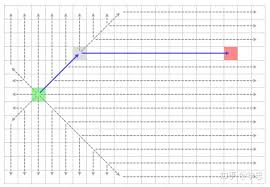
\includegraphics[width=0.3\textwidth]{jps.jpeg}}}
  \hspace{0.2em}
  \subfigure{\label{fig:schem_diag_prm}}\addtocounter{subfigure}{-2}
  \subfigure{\subfigure[PRM示意图]{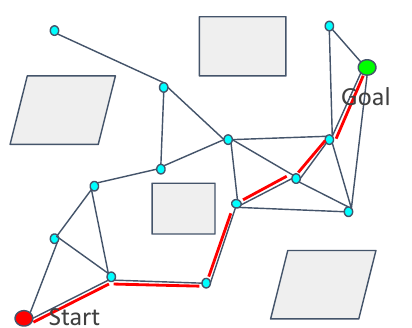
\includegraphics[width=0.3\textwidth]{prm.png}}}
  \hspace{0.2em}
  \subfigure{\label{fig:schem_diag_rrt}}\addtocounter{subfigure}{-2}
  \subfigure{\subfigure[RRT示意图]{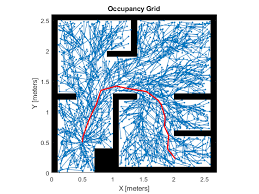
\includegraphics[width=0.3\textwidth]{rrt_2.png}}}
  \end{minipage}
  \caption{三种典型的路径搜索算法示意图\label{fig:three_methods_of_path_search}}
\end{figure}

本课题拟在$SE(3)$状态空间中为冗余驱动多旋翼飞行器搜索出一条可行路径,构型空间维度较高(6维)
且重点关注路径的安全性,并不优先考虑最优性,
故选择RRT算法作为前端路径搜索算法。
\subsection{$SE(3)$空间中的RRT算法}\label{subsec:rrt_in_SE3}
\subsubsection{RRT算法原理}\label{subsubsec:process_of_rrt}
如\ref{subsec:path_search_overview}节所述,RRT是一种通过随机构建空间填充树来高效搜索非凸高维空间的算法。
这棵树是以起始状态为根节点,根据从搜索空间中随机抽取的样本增量式构建的。
每次迭代都从搜索空间中采样出一个样本点,随后尝试从已有的树中距离样本点最近的节点向样本点以一定步长作延伸,到达一个新状态并形成一个运动基元,
如果该运动基元是有效的(比如全部位于无碰撞空间中,或满足某些其它的约束),则把这个运动基元和这个新状态分别作为边和节点加入树中,
这样整棵树就完成了一次生长。当新状态与目标状态的距离小于一定阈值且与目标状态的连接有效,则完成搜索。

本课题的$SE(3)$空间中的RRT算法完全遵循这些步骤,具体算法流程见算法\ref{alg:rrtse3}。

\begin{algorithm}[H]
  %\DontPrintSemicolon
  \wuhao
  \caption{$SE(3)$空间中的RRT算法\label{alg:rrtse3}}
  \begin{algorithmic}[1]
    \REQUIRE 地图$\mathcal{M}$、起始状态$\bm{x}_{init} \in SE(3)$、目标状态$\bm{x}_{goal} \in SE(3)$、\newline 
        最大迭代次数$n$、采样概率$p$和步长$\delta$ \\
    \ENSURE 从$\bm{x}_{init}$到$\bm{x}_{goal}$的一条可行路径$\varGamma$ \\
    \STATE 初始化搜索树$\mathcal{T}$,其中只有根节点$\bm{x}_{init}$ \\
    \FOR{$i = 1 \ to \ n$}
      \STATE 获得$\bm{x}_{sample}$:$\bm{x}_{sample}$有$p$的概率通过在搜索空间中均匀随机采样得到,有$(1-p)$的概率直接取$\bm{x}_{goal}$ \\
      \STATE 在搜索树$\mathcal{T}$中找到与$\bm{x}_{sample}$距离最近的节点$\bm{x}_{near}$ \\
      \STATE 从$\bm{x}_{near}$到$\bm{x}_{sample}$以步长$\delta$作插值,得到新状态$\bm{x}_{new}$ \\
      \IF {运动基元$(\bm{x}_{near} \rightarrow \bm{x}_{new})$无碰撞}
        \STATE 将$\bm{x}_{new}$作为新节点加入搜索树$\mathcal{T}$,并设置其父节点为$\bm{x}_{near}$\\
      \ENDIF
      \IF {$\bm{x}_{new}$与$\bm{x}_{goal}$之间的距离小于等于$\delta$且运动基元$(\bm{x}_{near} \rightarrow \bm{x}_{new})$无碰撞}
        \STATE 将$\bm{x}_{goal}$加入搜索树$\mathcal{T}$,并设置其父节点为$\bm{x}_{new}$ \\
        \STATE 从$\bm{x}_{goal}$根据父节点回溯出路径$\varGamma$ \\
        \STATE 结束循环 \\
      \ENDIF
    \ENDFOR
  \end{algorithmic}
\end{algorithm}

\subsubsection{$SE(3)$状态空间中的相关操作}\label{subsubsec:operations_in_SE3}
从算法\ref{alg:rrtse3}中可以看到,在搜索过程中需要对状态空间进行均匀采样,需要计算两个状态之间的距离,
在得到新状态以及对运动基元的有效性进行检测时还需要在两个状态之间进行插值。
即需要对$SE(3)$空间作采样、度量和插值三种操作。
$SE(3)$状态空间是一种复合的状态空间,由位置子空间$\mathbb{R}^3$和姿态子空间$SO(3)$构成,即$SE(3)=\mathbb{R}^3\times SO(3)$
在进行上述三种操作时可以先分别对两个子空间独立进行考虑,最后再进行整合。

位置子空间是欧几里得空间,在其中进行均匀采样就是分别对三个坐标值进行均匀采样;
两个位置之间的距离就是欧氏距离:
\begin{equation}
  \text{Dist}_{\mathbb{R}^3}(\bm{p}_1, \bm{p}_2) = \Vert \bm{p}_1 - \bm{p}_2 \Vert_2, \forall \bm{p}_1, \bm{p}_2 \in \mathbb{R}^3
  \label{equ:distance_in_R3}
\end{equation}
两个位置向量之间的线性插值如下式所示:
\begin{equation}
  \text{Interp}_{\mathbb{R}^3}(\bm{p}_1, \bm{p}_2; t) = 
  (1 - t)\bm{p}_1 + t\bm{p}_2, \forall \bm{p}_1, \bm{p}_2 \in \mathbb{R}^3, \forall t \in [0, 1]
  \label{equ:interpolation_in_R3}
\end{equation}

位置子空间中上述三种操作都很直接。
然而,在非欧的姿态子空间$SO(3)$中进行这些操作就显得不那么直观了。
一种比较朴素的做法是把$SO(3)$中的姿态用欧拉角表示,然后按$\mathbb{R}^3$空间中的方法来进行操作。
但是由于欧拉角的奇异性与周期性,使得欧氏空间中的度量方法并不能很好地反映姿态之间的差异。
比如,两组数值上差别很大的欧拉角可能表示的是两个相近甚至相同的姿态。
所以这种做法缺乏合理性。

\begin{figure}[ht]
  \centering
  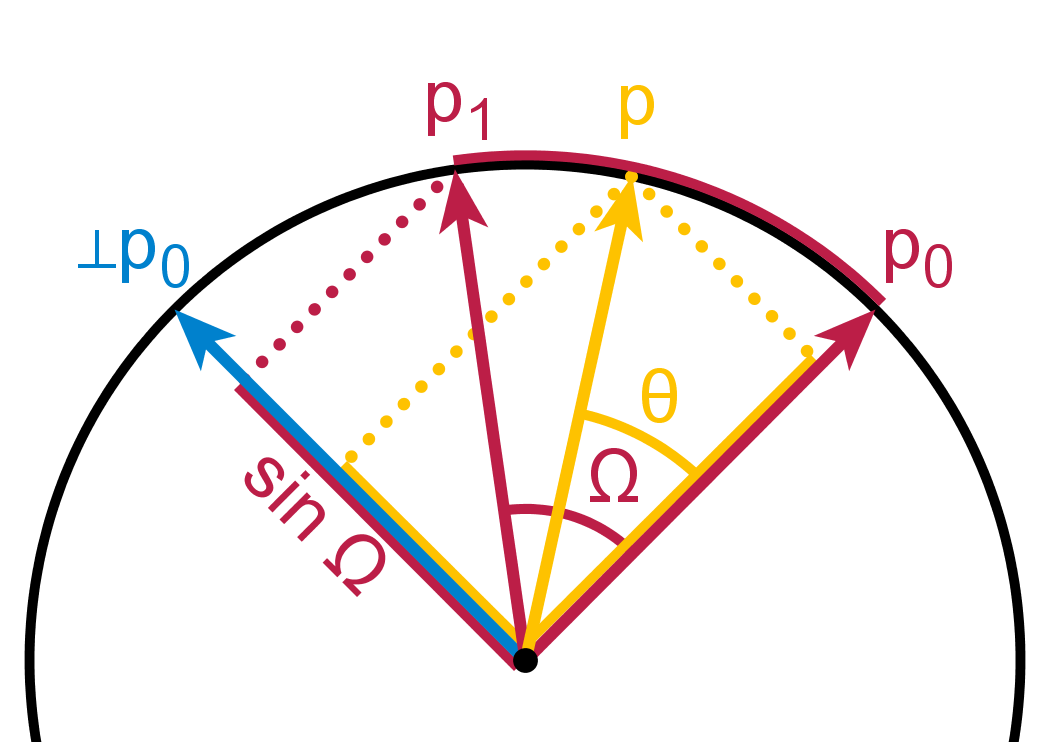
\includegraphics[width = 0.58\textwidth]{Slerp_factor_explanation.png}
  \caption{球面线性插值(slerp)示意图}
  \label{fig:slerp}
\end{figure}

本课题设计的RRT算法中对$SO(3)$空间的处理方式参考Kuffner等人于2004年提出的方法\cite{kuffner2004effective},
以上三种操作均基于四元数来进行,这样可以有效避免姿态表示的奇异性与重复性带来的缺点。
记表示绕轴$\bm{v} = \trans{[v_1 \quad v_2 \quad v_3]} \in \mathbb{R}^3$旋转角度$\theta \in \mathbb{R}$的单位四元数为:
\begin{equation}
  \bm{Q} = \trans{
    \begin{bmatrix}
      w & x & y & z
    \end{bmatrix}
  }
   = \trans{
     \begin{bmatrix}
       \cos{\frac{\theta}{2}} & v_1\cos{\frac{\theta}{2}} & v_2\cos{\frac{\theta}{2}} & v_3\cos{\frac{\theta}{2}}
     \end{bmatrix}
   }
   \label{equ:definition_of_unit_quaternion}
\end{equation}
则将在$SO(3)$空间中进行均匀采样可视为在单位四元数超球面上进行均匀采样,其流程如算法\ref{alg:uniform_unit_quaternion}所示;

\begin{algorithm}[H]
  \wuhao
  \caption{生成均匀分布的随机单位四元数\label{alg:uniform_unit_quaternion}}  
  \begin{algorithmic}[1] %每行显示行号  
      \REQUIRE 无  
      \ENSURE 均匀随机四元数$\bm{Q}=(w,x,y,z)$
      \STATE $s=uniform(0,1)$ // uniform(0,1)为生成0到1之间的均匀分布随机数
      \STATE $\sigma_{1}=\sqrt{1-s}$
      \STATE $\sigma_{2}=\sqrt{s}$
      \STATE $\theta_{1}=2\pi*uniform(0,1)$
      \STATE $\theta_{2}=2\pi*uniform(0,1)$
      \STATE $w=\cos(\theta_{2})*\sigma_{2}$
      \STATE $x=\sin(\theta_{1})*\sigma_{1}$
      \STATE $y=\cos(\theta_{1})*\sigma_{1}$
      \STATE $z=\sin(\theta_{2})*\sigma_{2}$
      \RETURN{$(w,x,y,z)$}
  \end{algorithmic}  
\end{algorithm} 

两个$SO(3)$状态间的距离定义为其在超球面上的弧长,即
\begin{equation}
  \text{Dist}_{SO(3)}(\bm{Q}_1, \bm{Q}_2) = \arccos(\trans{\bm{Q}_1}\bm{Q}_2), \forall \bm{Q}_1, \bm{Q}_2 \in SO(3)
  \label{equ:distance_in_SO3}
\end{equation}
在两个$SO(3)$状态间进行插值可视为在单位四元数超球面上进行球面线性插值(slerp,\figref{fig:slerp}),即:
\begin{equation}
  \text{Interp}_{SO(3)}(\bm{Q}_1, \bm{Q}_2; t) = 
  \frac{\sin[(1-t)\varOmega]}{\sin\varOmega}\bm{Q}_1 + \frac{\sin[t\varOmega]}{\sin\varOmega}\bm{Q}_2, 
  \forall \bm{Q}_1, \bm{Q}_2 \in SO(3), \forall t \in [0, 1]
  \label{equ:interpolation_in_SO3}
\end{equation}

现在已经分别确定了$SE(3)$中位置子空间和姿态子空间的采样、度量和插值的方法,
那么整个$SE(3)$空间中的采样和插值操作可以分别对其子空间进行,最后将得到的结果复合即可;
两个$SE(3)$状态的距离则可以表示如下:
\begin{equation}
  \text{Dist}_{SE(3)}(\bm{x}_1, \bm{x}_2) = 
  \sqrt{\text{Dist}_{\mathbb{R}^3}^2(\bm{p}_1, \bm{p}_2) + \text{Dist}_{SO(3)}^2(\bm{Q}_1, \bm{Q}_2)}, 
  \forall \bm{x}_1, \bm{x}_2 \in SE(3)
  \label{equ:distance_in_SE3}
\end{equation}
其中$\bm{p}_i \in \mathbb{R}^3$和$\bm{Q}_i \in SO(3)$分别为$\bm{x}_i \in SE(3)$的位置和姿态分量($i=1,2$)。
\subsection{近邻搜索}\label{subsuc:near_search}
RRT算法的另一个关键步骤是在已有的树中寻找出距离采样点$\bm{x}_{sample}$最近的节点,
这是一个近邻搜索问题,其耗时与待搜索集合中的元素个数$n$呈正相关,
也就是说,随着RRT算法迭代次数的增加,查找最近节点这一步的耗时也会随之增加,
所以这一步的效率是影响整个寻路算法效率的最重要因素之一。

近邻搜索最简单的方法就是线性搜索,其具有$O(n)$的时间复杂度。
显然,当$n$很大时线性搜索并不是一种高效的方法。
目前有许多用来存储带查找元素的数据结构可以加速搜索,
如Kd树\cite{bentley1975multidimensional}就是一种用来组织欧氏空间$\mathbb{R}^k$中点的数据结构,
在一棵平衡的Kd树中作最近邻搜索的平均时间复杂度为$O(\text{log}n)$;
1995年Brin提出的几何近邻搜索树(geometric near-neighbor access tree,GNAT)\cite{1995Near}只需要定义好距离函数就可以存储任意种类的数据点,
并且有相关实验能说明GNAT树在近邻搜索问题上的高效性。

根据本课题的需求,这里选择GNAT作为存储非欧空间$SE(3)$中点的数据结构。下面对GNAT的构建和基于GNAT的近邻搜索算法作简要介绍

\subsubsection{GNAT数据结构简介}\label{subsubsec:introduction_of_gnat}
GNAT是一种基于空间的分层超平面划分(hierarchical hyperplane partitioning)对度量空间(metric space)进行索引的数据结构。
在介绍GNAT的核心思想之前,先给出Dirichlet域的概念\cite{Engel1986}:
\begin{definition}[(Dirichlet域)]
  \label{def:dirichlet_domain}
  给定度量空间$M$,以及点集$P=\{\bm{x}_1,\cdots,\bm{x}_k\} \subset M$,
  点$\bm{x}_i \in P$的Dirichlet域$\mathbb{D}_{\bm{x}_i} \subset M$是$M$中所有满足下述条件的点$\bm{x}$的集合:
  \begin{equation}
    \text{Dist}(\bm{x}, \bm{x}_i) \leq \text{Dist}(\bm{x}_j,\bm{x}_i),\forall j \in \{1,\cdots,k\} \setminus \{i\}
    \label{condition_of_points_in_Dirichlet_domain}
  \end{equation}
\end{definition}

在GNAT树的根节点处,一系列分割点$X$被一种贪心策略从待存储的点集$S$中选出,
接着基于这些分割点将度量空间$M$划分为一系列Dirichlet域$\mathbb{D}_{\bm{x}_1},\cdots,\mathbb{D}_{\bm{x}_k}$,
剩下的点将根据它们落入的Dirichlet域分组,随后继续对这些分组重复上述步骤,最后递归地构建出GNAT。
\figref{fig:simple_gnat}展示了一棵简单的2层GNAT结构,
图中较大的点代表顶层节点(根节点)的分割点,较小的点代表子节点(叶节点)的分割点;
较粗的线代表顶层分割点对应区域的边界,而较细的线则代表底层分割点的。
\begin{figure}[ht]
  \centering
  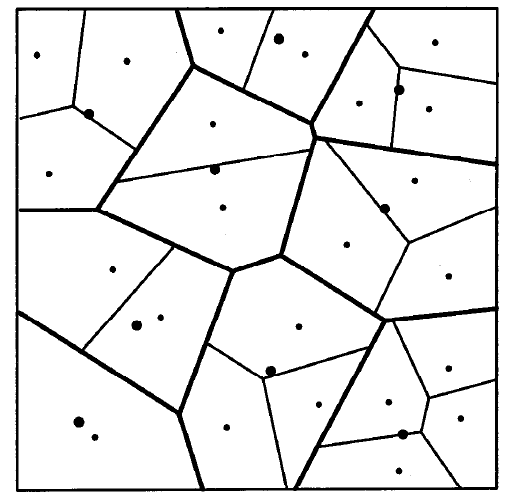
\includegraphics[width = 0.58\textwidth]{simple_gnat.png}
  \caption{一棵2层GNAT示意图}
  \label{fig:simple_gnat}
\end{figure}

GNAT树的基本构建过程叙述如下:
\begin{enumerate}
  \renewcommand{\labelenumi}{(\theenumi)}
  \item 从待组织的数据集中用贪心策略选出相隔足够远的$k$个分割点$\bm{x}_1,\cdots,\bm{x}_k$;
  \item 将数据集中剩下的点与最近的分割点相关联,并将与分割点$\bm{x}_i$相关联的点的集合记为$D_{\bm{x}_i}$;
  \item 对每对分割点$(\bm{x},\bm{x}_j)$,计算如下距离范围:
  \begin{equation}
    \text{range}(\bm{x_i}, D_{\bm{x}_j}) = [\text{minDist}_M(\bm{x_i}, D_{\bm{x}_j}), \text{maxDist}_M(\bm{x_i}, D_{\bm{x}_j})]
  \end{equation},用于搜索时的剪枝操作;
  \item 递归地对每个$D_{\bm{x}_i}$重复上述过程。
\end{enumerate}

\subsubsection{基于GNAT的近邻搜索}\label{subsubsec:near_search_based_on_gnat}
给定一个点$\bm{x}$,若要在GNAT中搜索出所有与$\bm{x}$的距离在$r$之内的所有点($r$-近邻点),
除了充分利用GNAT所表达的数据集的固有几何信息外,还可以利用距离信息进行剪枝以提高效率。
如\figref{fig:gnat_branch_prunning}所示,因为$\text{Dist}(\bm{x}, \bm{p}) + r < \text{min\_d}(\bm{p}, D_{\bm{p}_i})$,
所以$D_{\bm{p}_i}$中就一定不存在$\bm{x}$的$r$-近邻点,这样$D_{\bm{p}_i}$对应的子节点就可以被剪除。
\begin{figure}[ht]
  \centering
  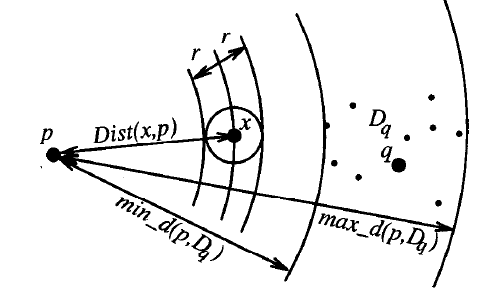
\includegraphics[width = 0.58\textwidth]{gnat_branch_prunning.png}
  \caption{利用距离信息在$r$-近邻搜索中进行剪枝的原理图}
  \label{fig:gnat_branch_prunning}
\end{figure}

在GNAT中进行$r$-近邻搜索的步骤叙述如下:
\begin{enumerate}
  \renewcommand{\labelenumi}{(\theenumi)}
  \item 记$P$为当前可能包含$\bm{x}$的$r$-近邻点的节点(初始状态下为根节点)的分割点,初始时$P$包含当前节点所有的分割点;
  \item 不重复地取一点$\bm{y} \in P$,若$\text{Dist}_M(\bm{x}, \bm{y}) \leq r$,则将$\bm{y}$加入结果中 \label{itm:pick_a_point_from_P};
  \item 考察所有$\bm{x}_i \in P$,如果有$[\text{Dist}_M(\bm{x}, \bm{y}_i)-r, \text{Dist}_M(\bm{x}, \bm{y}_i)+r] \cap \text{range}(\bm{y}, D_{\bm{x}_i}) = \emptyset$,则将$\bm{x}_i$从$P$中移除 \label{itm:prunning};
  \item 重复步骤\ref{itm:pick_a_point_from_P}和\ref{itm:prunning},直到$P$中所有点都试过一遍;
  \item 对$P$中剩下的所有点$\bm{y}_i$,递归地对$D_{\bm{y}_i}$进行搜索。
\end{enumerate}

如果要得到数据集中距离给定的$\bm{x}$最近的点,可以先基于Dirichlet域找到$\bm{x}$在GNAT中所在的叶节点,
随后在叶节点中线性搜索出其中距离$\bm{x}$最近的点,记这个最小距离为$r'$;
接着搜索出$\bm{x}$的所有$r'$-近邻点,
最后再对这些$r'$-近邻点进行线性搜索得到精确$\bm{x}$的最近邻。

为说明GNAT在近邻搜索上的高效性,本课题随机生成了$10^5$个Eigen三维双精度浮点型向量,分别基于线性搜索和GNAT做最近邻搜索。
经过数次集重复试验,每次都生成不同的随机点集,发现二者耗时均很稳定,
线性搜索平均耗时为34.6毫秒,而GNAT平均耗时仅为0.105毫秒,
二者相差数百倍,根据这个结果可以认为基于GNAT的近邻搜索之于线性搜索有巨大的优势。

以上介绍了基于GNAT的近邻搜索的通用方法,在本课题的应用场景中,
对应的度量空间$M$就是$SE(3)$空间,而GNAT所存储的就是当前的搜索树的所有节点。

\subsection{有效性检测}\label{subsec:validaty_checking}
在RRT算法中涉及两种有效性检测,一种是判断搜索空间中的单个状态是否有效,
另一种是基于单个状态的有效性检测来判断一个运动基元是否有效。

在本课题所设计的$SE(3)$空间的RRT算法(算法\ref{alg:rrtse3})中,
对状态和运动有效性的判断标准是其是否让飞行器与障碍物发生碰撞。
因为需要同时考虑飞行器的位置和姿态,且考虑到在狭小空间内实现轨迹规划的最终目标,
有必要在前端路径搜索时就考虑飞行器的形状。

\begin{figure}[ht]
  \centering
  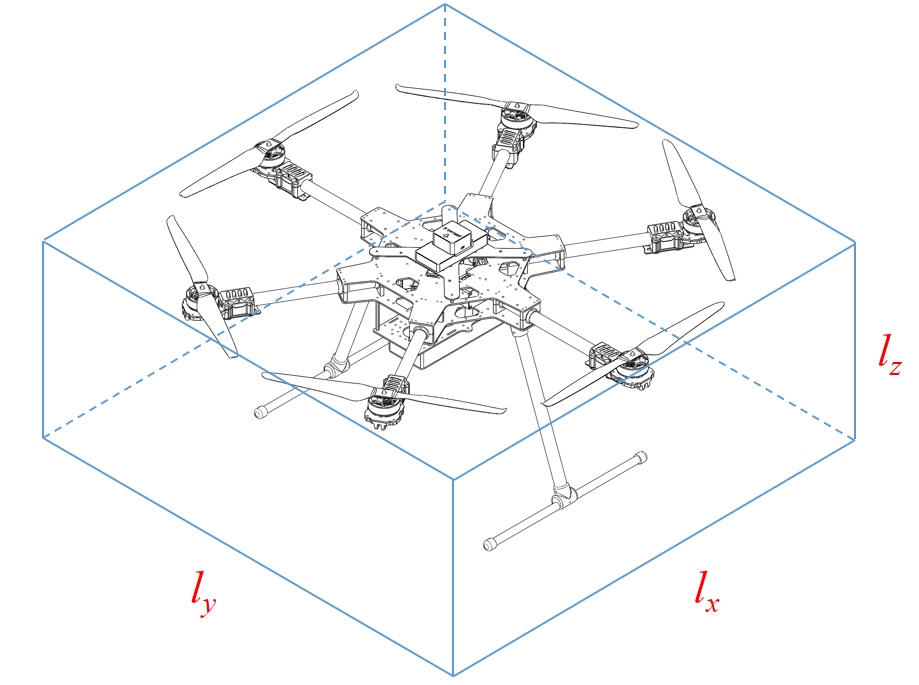
\includegraphics[width = 0.62\textwidth]{approximate_cuboid.png}
  \caption{将飞行器的形状近似为长方体}
  \label{fig:approximate_cuboid}
\end{figure}

如\figref{fig:approximate_cuboid}所示,这里将飞行器的形状简化为一个以其质心为中心、棱始终与机体坐标系保持一致的长方体。
则判断单个$SE(3)$状态是否有效,就转化为判断代表飞行器的长方体在这个状态对应的位置和姿态下是否与障碍物无交集,
而判断运动基元是否有效则可以在其上离散地取点(需要用到插值),若每个点对应的状态都是有效的,则认为该运动基元有效。
因此,本小节着重考虑单个状态的有效性检测。

在本课题所编写的RRT算法框架中,借鉴开源运动规划库OMPL\cite{sucan2012open}的思想,
将有效性检测这一操作抽象为StateValidityChecker和MotionValidityChecker两个抽象基类,
其中有纯虚函数isValid()作为提供给RRT算法主体的有效性检测公共接口,
如果要采用不同的有效性检测方法,只需继承StateValidityChecker或MotionValidityChecker抽象基类,实现其isValid()接口即可,
这样就实现了RRT算法主体与有效性检测的分离,提高了算法的复用性。

本课题根据地图形式的不同实现了基于点云的状态有效性检测和基于八叉树的状态有效性检测两种方法,
下面分别作简要说明。

\subsubsection{基于点云的状态有效性检测}\label{subsubsec:vc_based_on_pcl}
基于障碍物点云地图进行状态有效性检测的思路比较简单,
只要检查点云中是否有障碍物点落在给定$SE(3)$状态下的长方体内即可,有则无效,无则有效。
但如果单纯地使用线性搜索就必须要遍历整个点云,这对于稠密的点云来说非常的低效。
\begin{figure}[ht]
  \centering
  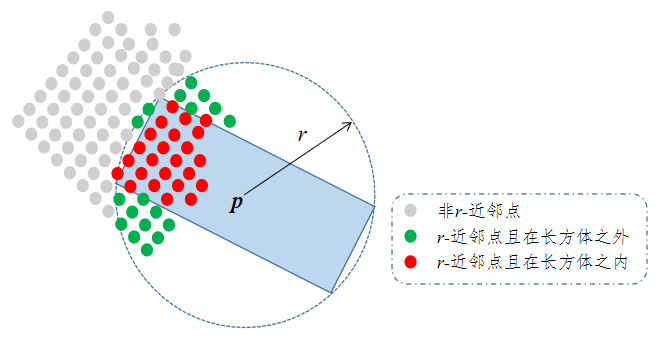
\includegraphics[width = 0.62\textwidth]{point_cloud_validity_checking.png}
  \caption{使用近邻搜索对有效性检测进行优化}
  \label{fig:point_cloud_validaty_checking}
\end{figure}

为解决这个问题,考虑使用GNAT数据结构来存储点云,配合近邻搜索来加速有效性检测过程。
如\figref{fig:point_cloud_validaty_checking}所示,长方体中心的位置为$\bm{p} \in \mathbb{R}^3$,
对$\bm{p}$进行近邻搜索得到其在点云中所有的$r$-近邻点,其中$r=\sqrt{l_x^2+l_y^2+l_z^2}/2$为长方体的外接球半径,
然后遍历所有$r$-近邻点检查是否有点位于长方体内,具体流程见算法\ref{alg:validaty_checking_based_on_point_cloud}。
\begin{algorithm}
  \wuhao
  \caption{基于障碍物点云的状态有效性检测\label{alg:validaty_checking_based_on_point_cloud}}  
  \begin{algorithmic}[1] %每行显示行号  
      \REQUIRE 用GNAT组织好的障碍物点云$\mathcal{P}$,待检测状态$\bm{x} \in SE(3)$, \newline
               长方体尺寸$(l_x, l_y, l_z)$,
               地图下界$\bm{b}_l \in \mathbb{R}^3$和上界$\bm{b}_u \in \mathbb{R}^3$
      \ENSURE 状态$\bm{x}$是否有效
      \STATE 计算长方体外接球半径$r=\sqrt{l_x^2+l_y^2+l_z^2}/2$
      \STATE 根据尺寸$(l_x, l_y, l_z)$和状态$\bm{x}$求出长方体各顶点的坐标$\bm{V}=[\bm{v}_1 \ \cdots \ \bm{v}_8]$
      \FOR {$i = 1 \ to \ 8$}
        \IF{$\bm{v}_i$超出地图上下界}
          \RETURN{False}
        \ENDIF
      \ENDFOR
      \STATE 在$\mathcal{P}$中搜索出长方体中心点$\bm{p}$($\bm{x}$的位置分量)的$r$-近邻点,构成点集$\mathcal{N}$
      \FORALL {$\bm{p}_{near} \in \mathcal{N}$}
        \IF{$\bm{p}_{near}$落在了长方体内}
          \RETURN{False}
        \ENDIF
      \ENDFOR
      \RETURN{True}
  \end{algorithmic}  
\end{algorithm} 

下面分析这种方法对有效性检测效率的改进程度。
令一次线性搜索有效性检测耗时为$T_1$,经由近邻搜索改进后的一次有效性检测耗时为$T_2$,
其中线性遍历检测整个点云耗时$T_{\text{linear}}$,使用GNAT获取$r$-近邻点耗时$T_{\text{GNAT}}$,线性遍历检测所有$r$-近邻点耗时$T_{r}$,
则有:
\begin{align}
  T_1 &\approx T_{\text{linear}} \label{equ:time_for_linear_validity_checking} \\
  T_2 &\approx T_{\text{GNAT}} + T_r \label{equ:time_for_optimized_validity_checking}
\end{align}
再令$T_{\text{GNAT}} = \lambda_1T_{\text{linear}}$,$T_r = \lambda_2T_{\text{linear}}$,
那么通常有$\lambda_1 \ll 1$,比如在\ref{subsubsec:near_search_based_on_gnat}节给出的例子中,就有$\lambda_1 < 1/300$;
$\lambda_2$近似为$r$-近邻点数量与点云中点的总数量的比值,通常也有$\lambda_2 \ll 1$,
故大多数情况下,$\lambda_1 + \lambda_2 \ll 1$,于是就有
\begin{equation}
  T_2 \approx (\lambda_1 + \lambda_2)T_1 \ll T_1
\end{equation}
这说明使用GNAT近邻搜索使有效性检测效率相比于暴力线性搜索有相当大的改进,
实际对比测试也支持这一结论。

\subsubsection{基于八叉树地图的状态有效性检测}\label{subsubsec:vc_based_on_pcl}
本课题中基于八叉树地图的状态有效性检测是通过调用FCL(flexible collision library)\cite{pan2012fcl}实现的。
FCL库提供了与八叉树地图库OctoMap\cite{hornung2013octomap}的接口,
可以很方便地检测不同几何形状(如代表飞行器的长方体)在不同位姿下与障碍物的碰撞。

\subsection{算法效果}\label{subsec:performance_of_rrtse3}
本小节展示所设计的$SE(3)$空间中的RRT算法使用基于点云和基于八叉树地图两种有效性检测方法的搜索效果,
并且每种方法都分别在障碍物稀疏及穿越狭窄通道两种场景下进行测试。测试中设置步长为0.8,采样概率为0.9。
\begin{figure}[!ht]
  \setlength{\subfigcapskip}{-1bp}
  \centering
  \begin{minipage}{\textwidth}

  \centering
  \subfigure{\label{fig:rrtse3_octomap_in_sparse_env_overview}}\addtocounter{subfigure}{-2}
  \subfigure{\subfigure[障碍稀疏(整体)]{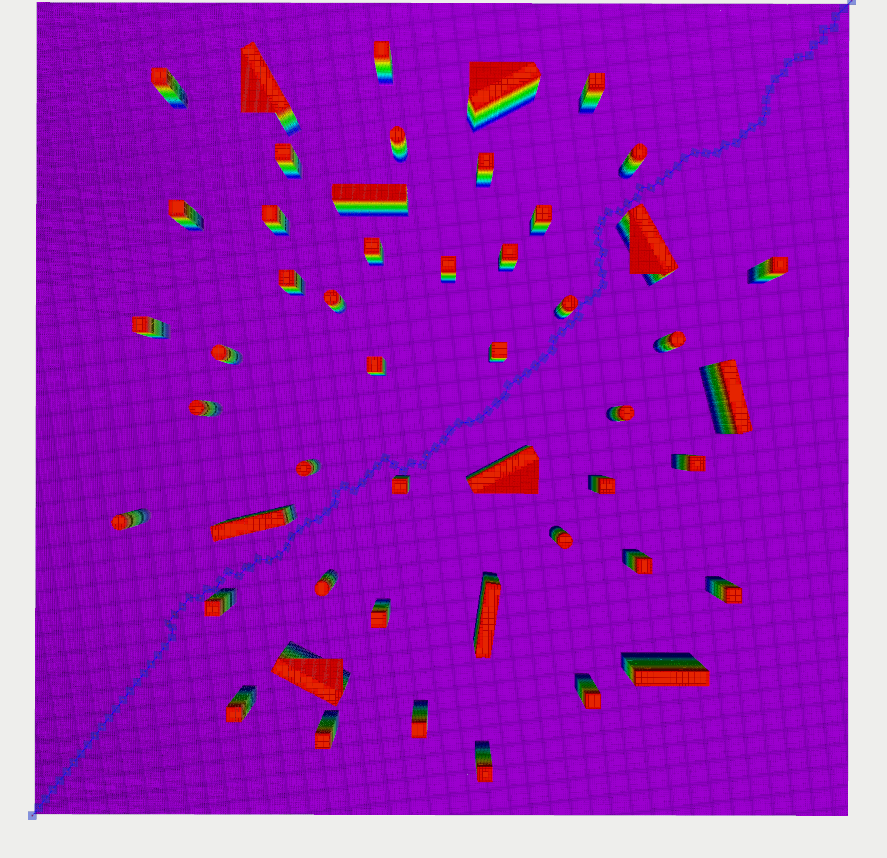
\includegraphics[width=0.23\textwidth]{octomap_rrtse3_1_overview.png}}}
  \hspace{0.2em}
  \subfigure{\label{fig:rrtse3_octomap_in_sparse_env_detail}}\addtocounter{subfigure}{-2}
  \subfigure{\subfigure[障碍稀疏(局部)]{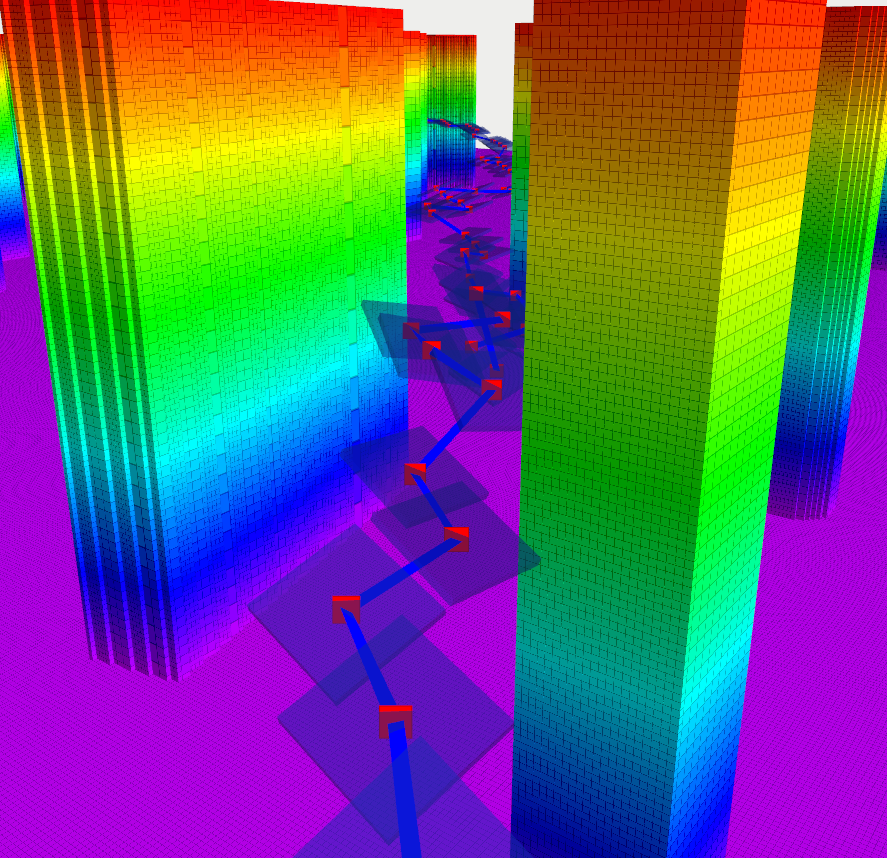
\includegraphics[width=0.23\textwidth]{octomap_rrtse3_1_detail.png}}}
  \hspace{0.2em}
  \subfigure{\label{fig:rrtse3_octomap_in_narrow_passage_overview}}\addtocounter{subfigure}{-2}
  \subfigure{\subfigure[狭窄通道(整体)]{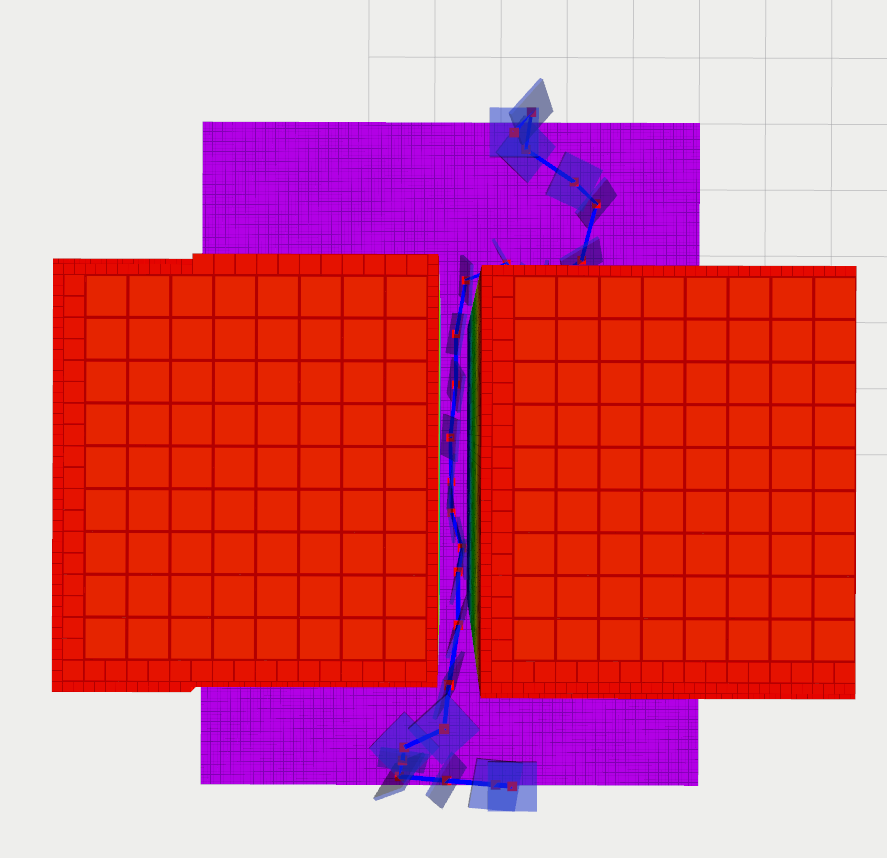
\includegraphics[width=0.23\textwidth]{octomap_rrtse3_2_overview.png}}}
  \hspace{0.2em}
  \subfigure{\label{fig:rrtse3_octomap_in_narrow_passage_detail}}\addtocounter{subfigure}{-2}
  \subfigure{\subfigure[狭窄通道(局部)]{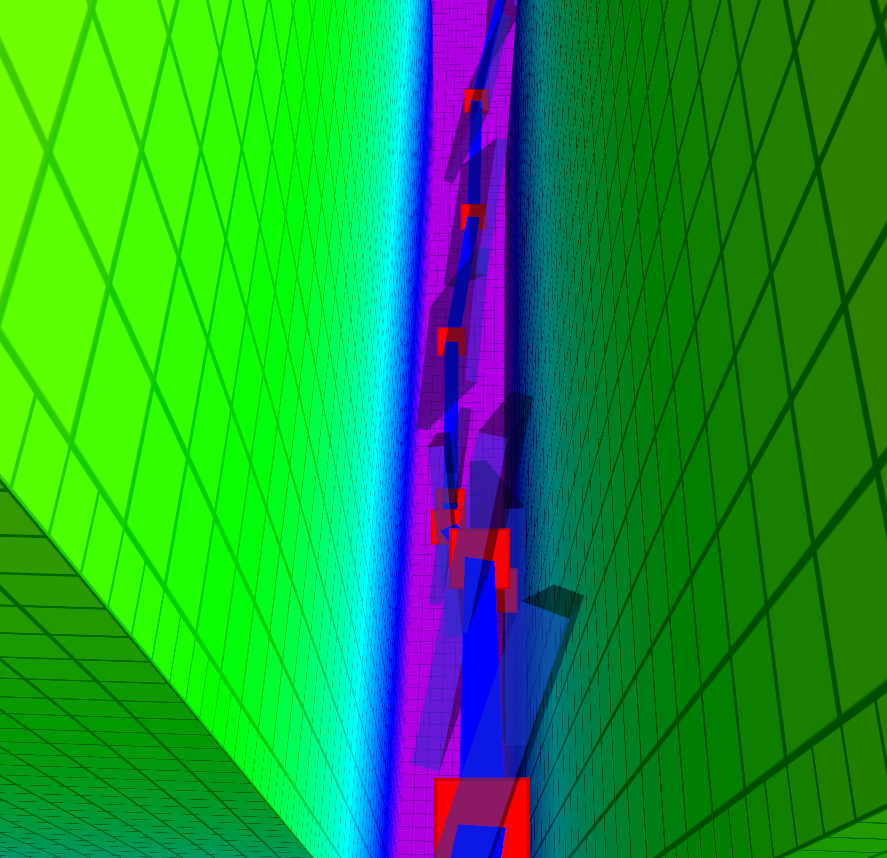
\includegraphics[width=0.23\textwidth]{octomap_rrtse3_2_detail.png}}}
  
  \end{minipage}
  \caption{$SE(3)$空间RRT算法效果可视化结果(基于八叉树地图)}
  \label{fig:performance_of_rrtse3_octomap}
\end{figure}

如\figref{fig:performance_of_rrtse3_octomap}所示为使用基于八叉树地图的有效性检测方法时的可视化结果。
图中蓝色半透明的长方体可视化表达了路径上每个$SE(3)$状态,
可见算法无论在宽松的环境中还是狭窄的环境中均能成功搜索出一条无碰撞路径,说明有效性检测成功发挥了其作用,
\figref{fig:rrtse3_octomap_in_narrow_passage_overview}中路径起点和终点附近的弯曲也表现出了RRT算法无法保证解的最优性的性质,
后续应用时将通过一定策略对路径点数量进行缩减来改善RRT的解中可能存在的这种局部的“舍近求远”现象。

\begin{figure}[!ht]
  \setlength{\subfigcapskip}{-1bp}
  \centering
  \begin{minipage}{\textwidth}

  \centering
  \subfigure{\label{fig:rrtse3_pcl_in_sparse_env_overview}}\addtocounter{subfigure}{-2}
  \subfigure{\subfigure[障碍稀疏(整体)]{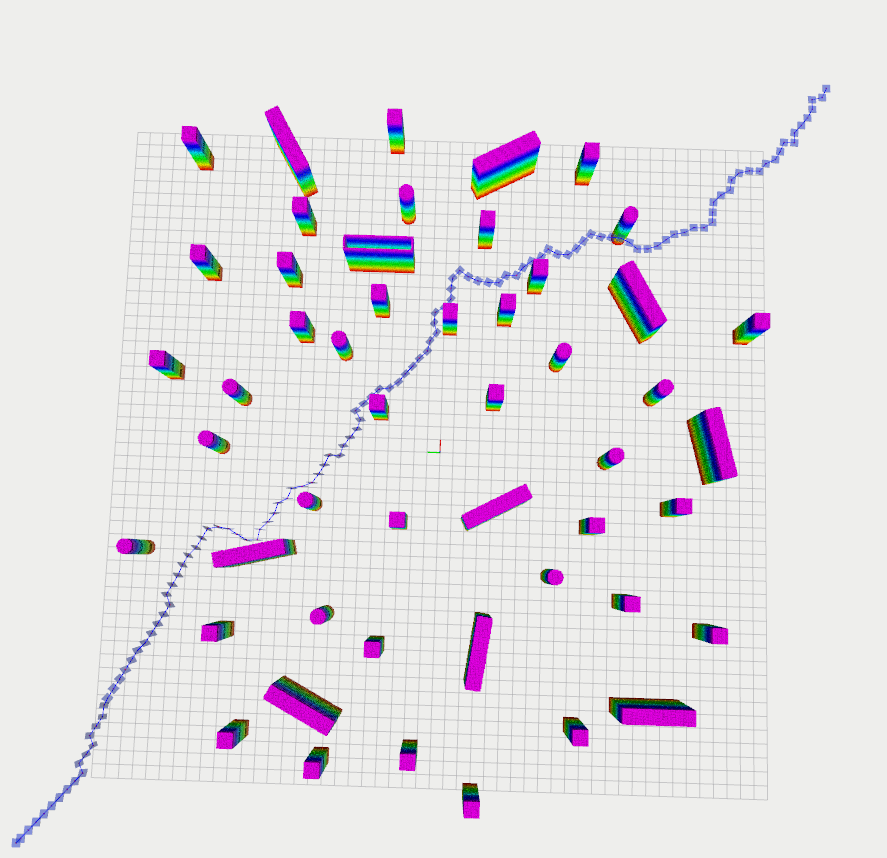
\includegraphics[width=0.23\textwidth]{point_cloud_rrtse3_1_overview.png}}}
  \hspace{0.2em}
  \subfigure{\label{fig:rrtse3_pcl_in_sparse_env_detail}}\addtocounter{subfigure}{-2}
  \subfigure{\subfigure[障碍稀疏(局部)]{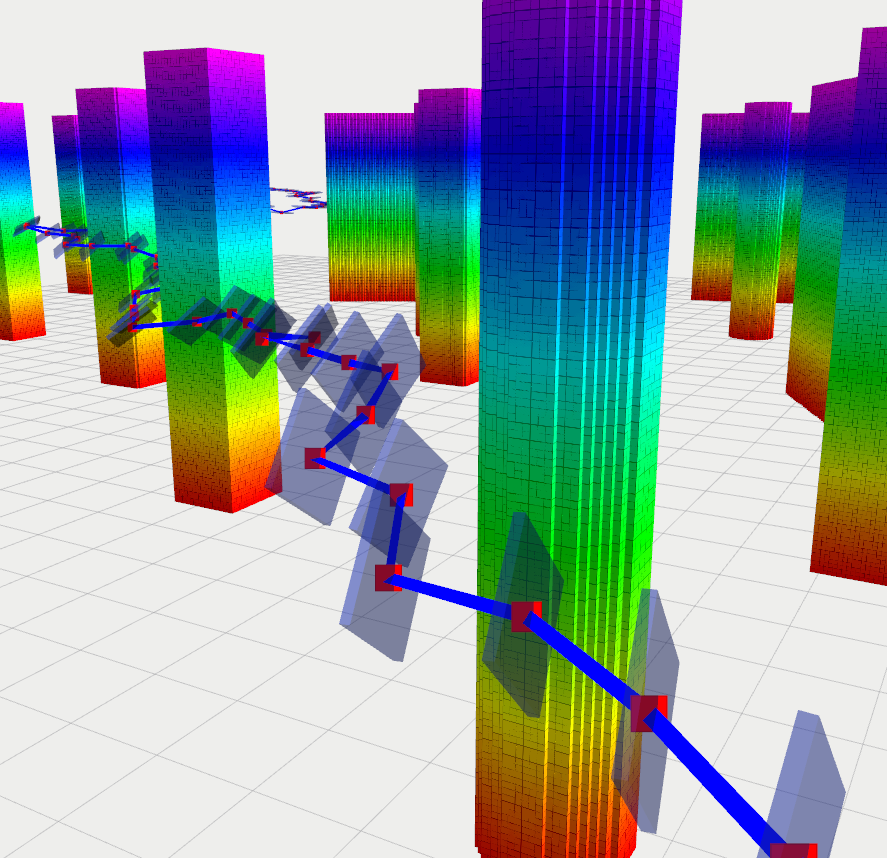
\includegraphics[width=0.23\textwidth]{point_cloud_rrtse3_1_detail.png}}}
  \hspace{0.2em}
  \subfigure{\label{fig:rrtse3_pcl_in_narrow_passage_overview}}\addtocounter{subfigure}{-2}
  \subfigure{\subfigure[狭窄通道(整体)]{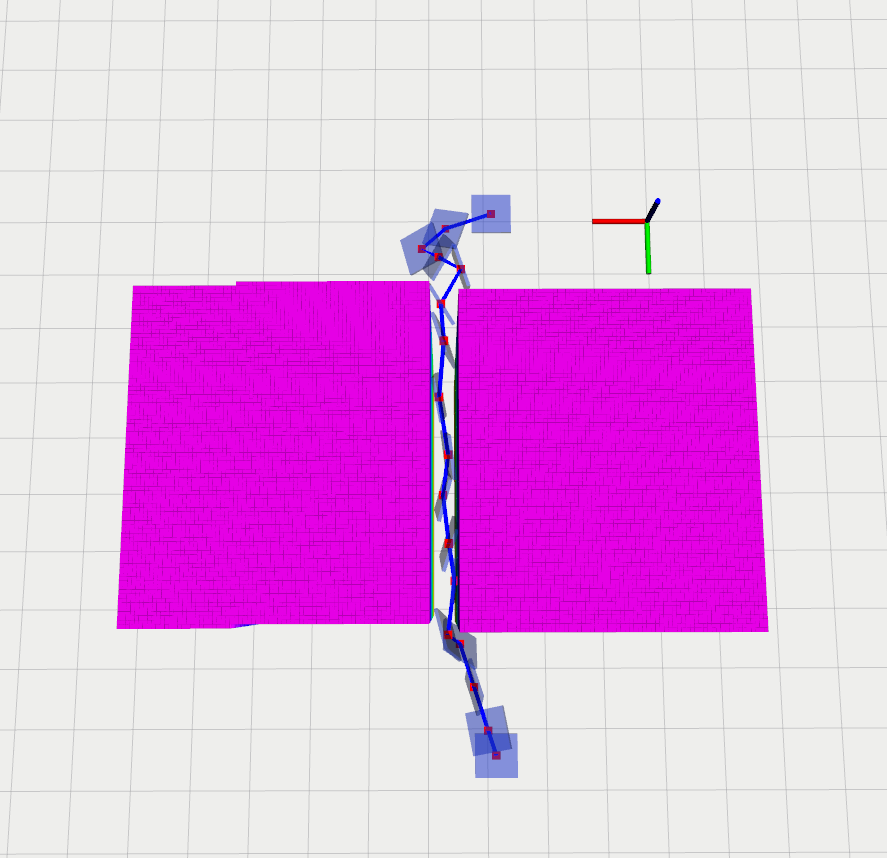
\includegraphics[width=0.23\textwidth]{point_cloud_rrtse3_2_overview.png}}}
  \hspace{0.2em}
  \subfigure{\label{fig:rrtse3_pcl_in_narrow_passage_detail}}\addtocounter{subfigure}{-2}
  \subfigure{\subfigure[狭窄通道(局部)]{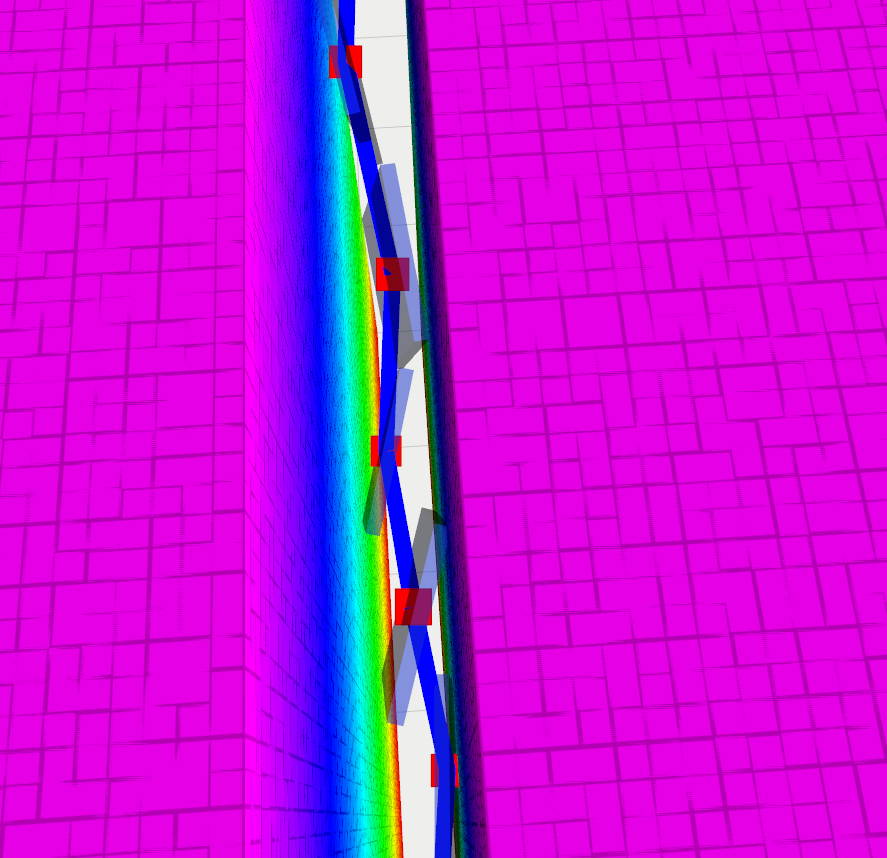
\includegraphics[width=0.23\textwidth]{point_cloud_rrtse3_2_detail.png}}}
  
  \end{minipage}
  \caption{$SE(3)$空间RRT算法效果可视化结果(基于点云地图)}
  \label{fig:performance_of_rrtse3_pcl}
\end{figure}

如\figref{fig:performance_of_rrtse3_pcl}所示为使用基于点云的有效性检测方法时的可视化结果,
可见得到的解与基于八叉树的方法并无很大区别。

\tabref{tab:rrtse3_performance_data}中列出了测试中所得到的一些数据。
可以看出狭窄环境的迭代次数要多于宽松的环境,
这是因为狭窄环境中可行区域占比更小,在一定迭代次数内找到解的概率就会更低。
而且可以注意到,同样环境和起终点条件下,
使用点云方法的求解时间显著高于使用八叉树方法,
这是由于这里的点云地图中障碍物内部也被填充,导致点的数量异常庞大,极大地增加了有效性检测的负担;
而基于八叉树的方法检测只需要用到障碍物表面信息。
如果在生成点云时能够合理地控制点的数量,尽量剔除冗余点,就能使点云法的求解速度大大提高;
在后文中所用到的一个50m$\times$50m大小、障碍物较为稠密的随机地图中,使用点云法可以在数百毫秒内搜索出一条对角路径。
另外,利用OctoMap库和PCL库\cite{rusu20113d}可以很方便地在点云和八叉树之间进行转换,
可以根据实际需求灵活地选择地图形式。

\begin{table}[htbp]
  \caption{关于$SE(3)$空间RRT算法的一些数据\label{tab:rrtse3_performance_data}}
  \vspace{0.5em}\centering\wuhao
  \begin{tabular}{ccccccc}
  \toprule[1.5pt]
  环境 & 地图类型 & 地图尺寸(m) & 起点(m) & 终点(m) & 迭代次数数量级 & 平均耗时\\
  \midrule[0.2pt]
  宽松 & 八叉树 & $60\times60\times6$ & $(29, -29, 3)$ & $(-29, 29, 3)$ & $10^2$ & 20毫秒左右\\
  宽松 & 点云 & $60\times60\times6$ & $(29, -29, 3)$ & $(-29, 29, 3)$ & $10^2$ & 数秒\\
  狭窄 & 八叉树 & $7.5\times10\times6$  & $(3, 1, 3)$ & $(3, 9, 3)$ & $10^3$ & 200毫秒以内\\
  狭窄 & 点云 & $7.5\times10\times6$  & $(3, 1, 3)$ & $(3, 9, 3)$ & $10^3$ & 数十秒\\
  \bottomrule[1.5pt]
  \end{tabular}
\end{table}

\section{3D安全飞行走廊生成算法的设计}\label{sec:sfc_gen_algorithm}
3D空间中的安全飞行走廊(SFC)一般用来描述无障碍物的空闲空间(free space),
一般用一系列球或凸多面体来表示,在无人机的轨迹规划中取得了许多应用\cite{han2021fast,mohta2018fast,gao2019flying}。
SFC通常在轨迹规划框架的前端部分根据初始路径生成,然后作为轨迹优化的约束给到后端。
目前SFC的生成方法也有多种,如Liu等人的RILS算法\cite{2017Planning}、Deits等人的IRIS方法\cite{deits2015computing}等。
本课题使用前者,下面对其进行简要介绍。
\subsection{算法原理}\label{subsec:design_of_sfc_gen_algorithm}
记障碍物点云为$\mathcal{O}$,本算法对$\mathbb{R}^3$空间进行操作,只需要$SE(3)$路径的位置部分,
记无碰撞位置路径为$P = \langle \bm{p}_0 \rightarrow \cdots \rightarrow \bm{p}_s \rangle$,
则算法将在每条线段$L_i = \langle \bm{p}_i \rightarrow \bm{p}_{i+1} \rangle$周围生成一个包含无碰撞空间的凸多面体$P_i$,
此过程分为两步,简述如下:
\subsubsection{无碰撞椭球的生成}
\begin{figure}[ht]
  \centering
  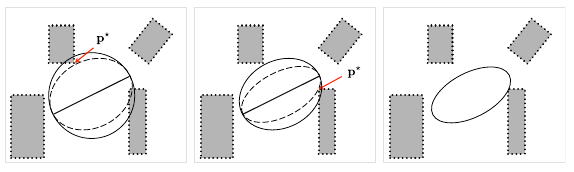
\includegraphics[width = 0.83\textwidth]{get_ellipsoid.png}
  \caption{生成无碰撞椭球示意图}
  \label{fig:get_ellipsoid}
\end{figure}
一个椭球$\xi$可以表示为如下形式:
\begin{equation}
  \xi(\bm{E}, \bm{d}) = \{\bm{p} = \bm{E}\bar{\bm{p}} + \bm{d} \mid \Vert \bar{\bm{p}} \Vert \leq 1 \}
  \label{equ:representation_of_ellipsoids}
\end{equation}

对于一个$\mathbb{R}^3$中的椭球来说,变换矩阵$\bm{E}$可以分解为旋转变换加缩放变换,即:
\begin{equation}
  \bm{E} = \trans{\bm{R}}\bm{S}\bm{R} = \trans{\bm{R}}\text{diag}(a, b, c)\bm{R}
  \label{equ:decomp_E}
\end{equation}
其中$a, b, c$分别为椭球坐标系的$\tilde{x}, \tilde{y}, \tilde{z}$轴对应的缩放系数。
任意一点到椭球的距离定义如\equref{equ:distance_to_ellipsoids},若$\rho(\bm{p}, \xi) < 1$,则$\bm{p}$位于椭球内部。
\begin{equation}
  \rho(\bm{p}, \xi(\bm{E}, \bm{d})) = \Vert \bar{\bm{p}} \Vert = 
  \Vert \bm{E}^{-1}(\bm{p} - \bm{d}) \Vert
  \label{equ:distance_to_ellipsoids}
\end{equation}

求线段$L$的无碰撞椭球即是令$\bm{d}$为线段的中点,固定椭球$\tilde{x}$轴与$L$重合且$2a=L$,
改变$b$和$c$得到一个尽可能大的、不包含障碍物点的椭球。
如\figref{fig:get_ellipsoid}所示,这个过程是一个从初始球体开始迭代收缩的过程,
具体流程如算法\ref{alg:generate_ellipsoid}所示。

\begin{algorithm}[h]
      \wuhao
      \caption{生成无碰撞椭球\label{alg:generate_ellipsoid}}  
      \begin{algorithmic}[1] %每行显示行号  
          \REQUIRE 线段$L_{i}= \langle \bm{p}_{i} \rightarrow \bm{p}_{i+1} \rangle $,障碍物点集$O$
          \ENSURE 无碰撞椭球$\xi$
          \STATE 初始化$\xi$为以$L_{i}$为直径的球体,且以$\bm{p}_{i}\bm{p}_{i+1}$为$\xi$的$\widetilde{x}$轴
          \STATE  $O_{inside}\gets \xi.getInside(O)$
          \WHILE {$O_{inside} \neq \emptyset$}
            \STATE $\bm{p}\gets \min_{\bm{q} \in O_{inside}}\Vert \bm{E}^{-1}(\bm{p}-\bm{d}) \Vert$
            \STATE 保持$\widetilde{x}$轴不变,$b=c$,调整$\xi$使其的边界经过点$\bm{p}$
            \STATE $O_{inside}\gets \xi.getInside(O)$
          \ENDWHILE
          \STATE 此时$\xi$接触一障碍物点$\bm{p}^{*}$,将其与$\xi$的$\widetilde{x}$轴确定的平面定为$\xi$的$\widetilde{x}-\widetilde{y}$平面
          \STATE 沿$\widetilde{z}$轴调整$\xi$使$c=a$
          \STATE  $O_{inside}\gets \xi.getInside(O)$
          \WHILE {$O_{inside} \neq \emptyset$}
            \STATE $\bm{p}\gets \min_{\bm{q} \in O_{inside}}\Vert \bm{E}^{-1}(\bm{p}-\bm{d}) \Vert$
            \STATE 沿$\widetilde{z}$轴调整$\xi$使其的边界经过点$\bm{p}$
            \STATE $O_{inside}\gets \xi.getInside(O)$
          \ENDWHILE
          \RETURN $\xi$
      \end{algorithmic}  
\end{algorithm} 

\subsubsection{凸多面体的生成}
\begin{figure}[ht]
  \centering
  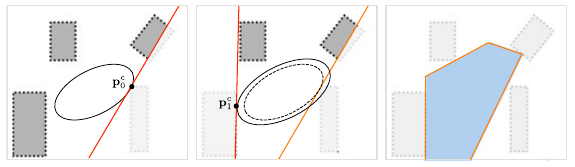
\includegraphics[width = 0.83\textwidth]{get_polyhedron.png}
  \caption{生成无碰撞无碰撞凸多面体示意图}
  \label{fig:get_polyhedron}
\end{figure}
如\figref{fig:get_polyhedron}所示,此过程也是通过一步步迭代,对之前生成的无碰撞椭球进行膨胀来得到最终的无碰撞凸多面体的,
具体流程见算法\ref{alg:generate_polyhedron}。
这里将第$i$步膨胀得到的半空间(halfspace)记作:
\begin{equation}
  H_i = \{\bm{p} \mid \trans{\bm{a}_i}\bm{p} < b_i\}
  \label{equ:halfspace_i}
\end{equation}

记最后得到的由$(m+1)$个半空间所确定的凸多面体为:
\begin{equation}
  \mathcal{P}(\bm{A}, \bm{b}) = \bigcap_{i=0}^m H_i = \{\bm{p} \mid \trans{\bm{A}}\bm{p} \prec \bm{b}\}, \bm{A} \in \mathbb{R}^{3\times m},\bm{b} \in \mathbb{R}^m
\end{equation}
\begin{algorithm}[h]
      \wuhao
      \caption{膨胀椭球生成无碰撞凸多面体\label{alg:generate_polyhedron}}  
      \begin{algorithmic}[1] %每行显示行号  
          \REQUIRE 无碰撞椭球$\xi^{0}(\bm{E},\bm{d})$,障碍物点集$O$ 
          \ENSURE 凸多面体$\mathcal{P}(\bm{A},\bm{b})$
          \STATE  $O_{remain}\gets \xi.getInside(O),j \gets 0$
    \WHILE {$O_{remain} \neq \emptyset$}
      \STATE $\bm{p}_{j}^{c} \gets \min_{\bm{q} \in O_{inside}}\Vert \bm{E}^{-1}(\bm{p}-\bm{d}) \Vert$ 
      \STATE 按比例膨胀$\xi^{0}$使其表面经过$\bm{p}_{j}^{c}$
      \STATE $\bm{a}_{j} \gets 2\bm{E}^{-1}\bm{E}^{-\text{T}}(\bm{p}_{j}^{c}-\bm{d})$
      \STATE $b_{j} \gets \bm{a}_{j}^{\text{T}}\bm{p}_{j}^{c}$
      \STATE 去除$O_{remain}$中不在半空间$H_{j}(\bm{a}_{j},b_{j})$之内的所有点
      \STATE $j \gets j+1$
    \ENDWHILE
    \STATE $\bm{A} \gets [\bm{a}_{0}\ \bm{a}_{1}\ \cdots]^{\text{T}}$,$\bm{b} \gets [b_0 \ b_1 \ \cdots]^{\text{T}}$
    \RETURN $\mathcal{P}(\bm{A},\bm{b})$
      \end{algorithmic}  
\end{algorithm} 

\subsection{效果展示}\label{subsec:impl_of_sfc_gen_algorithm}
如\figref{fig:sfc_generation}所示为SFC生成算法的运行结果的可视化示意图。
所使用的地图即是前述RRT测试所使用的宽松环境。
可以从图中清晰地看到每段路径周围的无碰撞椭球和在这些无碰撞椭球的基础上生成的凸多面体。
附近没有障碍物的路径段所生成的椭球保持初始的球形,而附近由障碍物的路径段所生成的椭球则被“压扁”;
所有凸多面体串成整个安全飞行走廊,注意这里加入了局部包围框(即一些额外的半空间),
以将飞行走廊限制在路径周围一定范围内。

在效率方面,该算法具有可观的计算速度,类似图中的飞行走廊的生成耗时在数十毫秒到百毫秒以内,
当然,耗时也会与点云中点的数量呈一定正相关。

\begin{figure}[!ht]
  \setlength{\subfigcapskip}{-1bp}
  \centering
  \begin{minipage}{\textwidth}

  \centering
  \subfigure{\label{fig:sfc_overview}}\addtocounter{subfigure}{-2}
  \subfigure{\subfigure[完整的SFC]{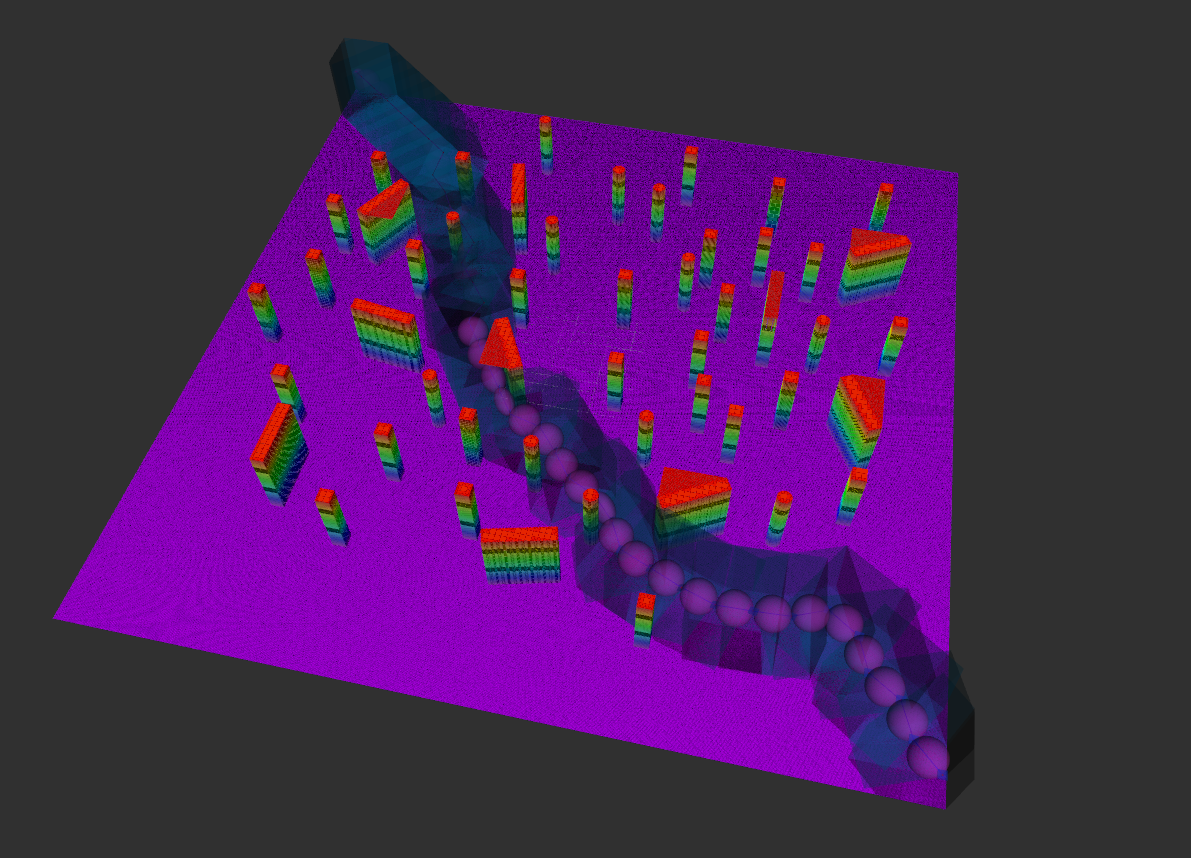
\includegraphics[width=0.3\textwidth]{octomap_sfc_overview.png}}}
  \hspace{0.2em}
  \subfigure{\label{fig:sfc_detail_1}}\addtocounter{subfigure}{-2}
  \subfigure{\subfigure[局部细节1]{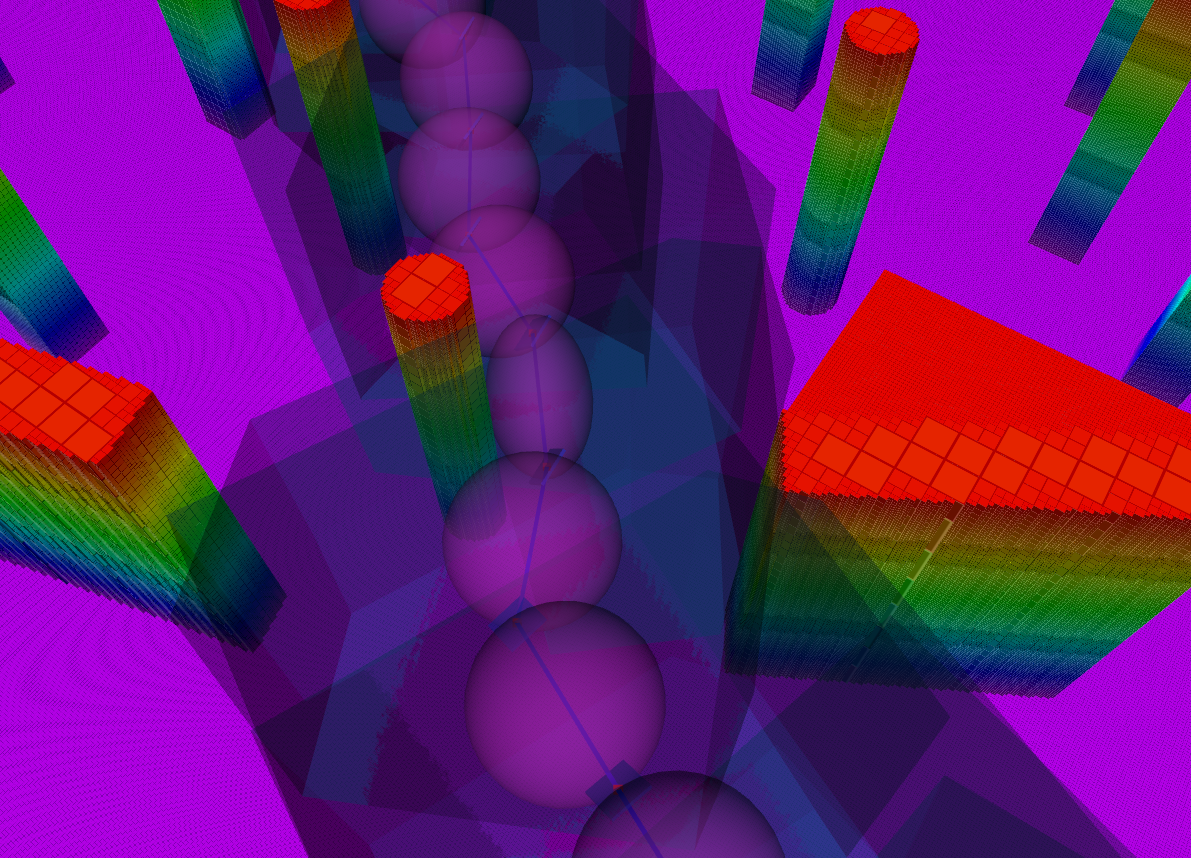
\includegraphics[width=0.3\textwidth]{octomap_sfc_detail_1.png}}}
  \hspace{0.2em}
  \subfigure{\label{fig:sfc_detail_2}}\addtocounter{subfigure}{-2}
  \subfigure{\subfigure[局部细节2]{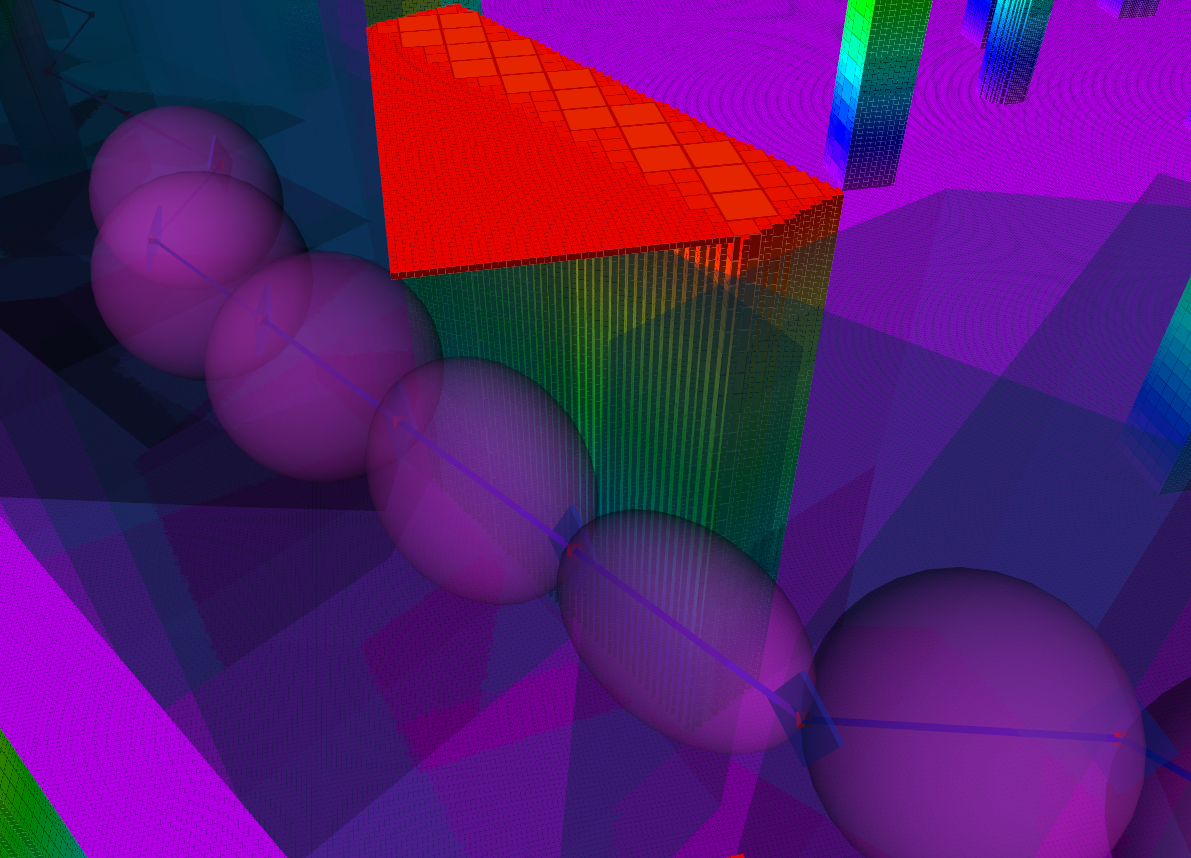
\includegraphics[width=0.3\textwidth]{octomap_sfc_detail_2.png}}}
  
  \end{minipage}
  \caption{SFC生成示意图}
  \label{fig:sfc_generation}
\end{figure}
\section{本章小结}\label{sec:summary_3}
本章首先对$SE(3)$空间中的RRT算法进行设计,
确定了$SE(3)$状态空间中的采样、插值和度量等操作,
介绍了用于近邻搜索的GNAT数据结构,
设计了基于点云地图和基于八叉树地图的两种有效性检测方法,
并对设计好的RRT算法进行了效果测试及分析;
随后设计并实现了安全飞行走廊的生成算法,并给出了实测效果。
综上所述,本章完成了对轨迹规划前端算法的设计与实现,
为后端部分提供了可行路径和安全约束等初始信息。
